\chapter{Programación PLC}
\label{ch:progPLC}
Como se prensento en el capitulo \ref{ch:intro} de este informe el material a utilizar
para poder alcanzar los objetivos. En el presente capítulo se describe el algoritmo 
de programación del programa que se grabo en el \gls{plc} 
\section{Algoritmo}
\label{sec:Algoritmo}

\begin{algorithm}[H]
 \KwData{this text}
 \KwResult{how to write algorithm with \LaTeX2e }
 initialization\;
 \While{not at end of this document}{
  read current\;
  \eIf{understand}{
   go to next section\;
   current section becomes this one\;
   }{
   go back to the beginning of current section\;
  }
 }
 \caption{How to write algorithms}
\end{algorithm}




\section{Programación}
\label{sec:Programacion}
Se utilizó el programa Twido Soft para poder programar el \gls{plc}. Se programó
en lenguaje Ladder.

El software Twido Soft sirve tanto como para enviar el programa al \gls{plc}, así como 
para descargar el programa que esta en el \gls{plc}. A tal efecto a continuación 
se explicaran algunas cualidades del programa para que sea simple su comprensión.

Lo primero que se presenta son la acción realizada en cada RUNG (pasos del programa).

\usetikzlibrary{trees}
\tikzstyle{every node}=[draw=black,thick,anchor=west,inner sep=2pt,minimum size=1pt]
\tikzstyle{selected}=[draw=cyan,fill=cyan!30]
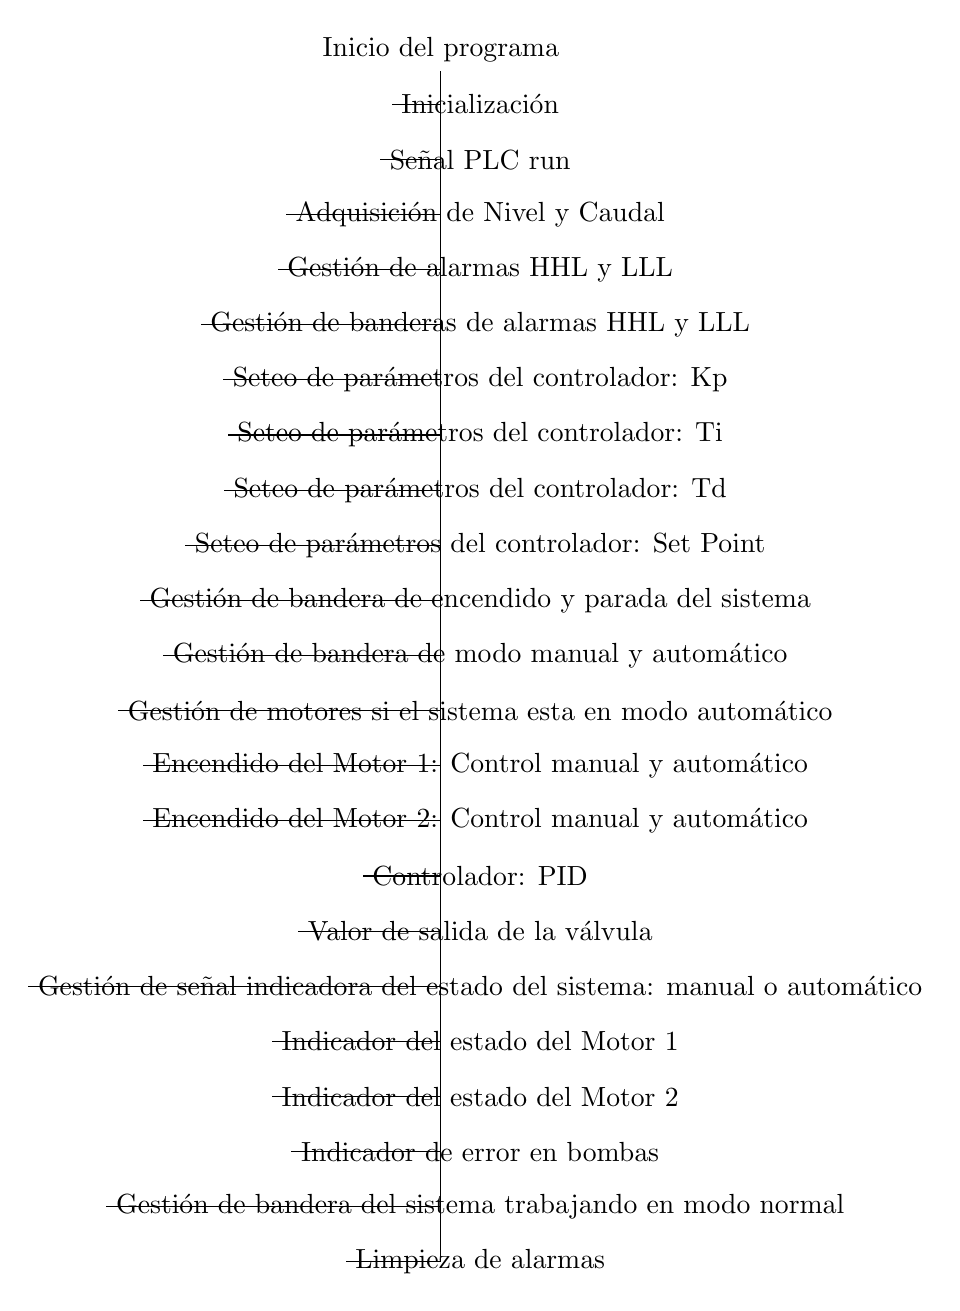
\begin{tikzpicture}[
  grow via three points={one child at (0.5,-0.7) and
  two children at (0.5,-0.7) and (0.5,-1.4)},   
  edge from parent path={(\tikzparentnode.south) |- (\tikzchildnode.west)}]
  \node (init) {Inicio del programa  }
    child { node {Inicialización} }
    child { node {Señal PLC run}    }
    child { node {Adquisición de Nivel y Caudal}    }
    child { node {Gestión de alarmas HHL y LLL}    }
    child { node {Gestión de banderas de alarmas HHL y LLL}    }
    child { node {Seteo de parámetros del controlador: Kp}    }
    child { node {Seteo de parámetros del controlador: Ti}    }
    child { node {Seteo de parámetros del controlador: Td}    }
    child { node {Seteo de parámetros del controlador: Set Point}    }
    child { node {Gestión de bandera de encendido y parada del sistema}    }
    child { node {Gestión de bandera de modo manual y automático}    }
    child { node {Gestión de motores si el sistema esta en modo automático}    }
    child { node {Encendido del Motor 1: Control manual y automático}    }
    child { node {Encendido del Motor 2: Control manual y automático}    }
    child { node {Controlador: PID}    }
    child { node {Valor de salida de la válvula}    }
    child { node {Gestión de señal indicadora del estado del sistema: manual o automático}    }
    child { node {Indicador del estado del Motor 1}    }
    child { node {Indicador del estado del Motor 2}    }
    child { node {Indicador de error en bombas}    }
    child { node {Gestión de bandera del sistema trabajando en modo normal}    }
    child { node {Limpieza de alarmas}    };
  
\end{tikzpicture}
\tikzstyle{every node}=[] % resets borders of tables
\tikzstyle{selected}=[] % resets selected
\todo{Anexo de lo que imprimimos desde el twido soft}


El programa presenta baderas que nos sirven para conocer diferentes estados
de la planta. En la tabla \ref{table:Banderasinternas} se pueden ver el nombre 
de las mismas y sus funciones.


\begin{table}[!t]

\renewcommand{\arraystretch}{1.3}
\centering
\begin{tabular}{c||c}
\hline
\bfseries Memoria & \bfseries Descripción\\
\hline \hline
\verb|M0|  & Bandera de inicialización\\
\verb|M1|  & Sistema Encendido/Apagado\\
\verb|M2|  & Sistema en modo Manual/Automático\\
\verb|M3|  & Error de Nivel\\
\verb|M4|  & Error de Motor\\
\hline
\end{tabular}
\caption{Banderas internas}
\label{table:Banderasinternas}
\end{table}

Por ultimo se expresan las entradas y salidas al \gls{plc}, tanto analógicas
como discretas en la tabla \ref{table:entradassalidas}.

\begin{table}[!t]

\renewcommand{\arraystretch}{1.3}
\centering
\begin{tabular}{c||c}
\hline
\bfseries Memoria & \bfseries Descripción\\
\hline \hline
\verb|Q0.0|  & Encender motor 1\\
\verb|Q0.1|  & Encender motor 2\\
\verb|Q0.7|  & Señal de encendido de los motores\\
\verb|I0.0|  & Retroalimentación desde el relevo térmico motor 1\\
\verb|I0.1|  & Retroalimentación desde el relevo térmico motor 2\\
\verb|IW0.1.0|  & Señal analógica de nivel\\
\verb|IW0.1.1|  & Señal analógica de caudal \\
\verb|QW0.1.0|  & Señal analógica de salida de apertura de la válvula \\
\hline
\end{tabular}
\caption{Entradas y salidas al PLC}
\label{table:entradassalidas}
\end{table}

\section{Comunicación}
\label{sec:Comunicacion}

Para ser capaces de interactuar con la aplicación de \gls{scada} definimos
ciertas palabras que nos permiten realizar acciones en el sistema y conocer
el estado del mismo.

La tabla \ref{table:bitlecturasescrituras} presenta dos palabras de dieciséis
bits, \verb|MW0| y \verb|MW1|, la primera de ella presenta bits de lectura, en donde se
refleja el estado del la plata, mientras que la segunda palabra sus bits son
de escritura y nos da la posibilidad de manejar la planta.
\begin{table}[!t]

\renewcommand{\arraystretch}{1.3}
\centering
\begin{tabular}{c||c||c||c}
\hline
\bfseries Tipo & \bfseries Word & \bfseries Bit & \bfseries Descripción\\
\hline \hline
Lect & \verb|MW0| & \verb|X0| & Señal Run PLC\\
Lect & & \verb|X1| & Alarma HHL\\
Lect & & \verb|X2|& Alarma LLL\\
Lect & & \verb|X3|& Alarma HL\\
Lect & & \verb|X4|& Alarma LL\\
Lect & & \verb|X5|& Error en motores (era \verb|MW0:X13|)\\
Lect & & \verb|X6|& Motor 1 encendido (era \verb|MW0:X11|)\\
Lect & & \verb|X7|& Motor 2 encendido(era \verb|MW0:X12|)\\
Lect & & \verb|X8|& Modo manual activado (era \verb|MW0:X14|)\\
Lect & & \verb|X9|& Modo automático activado y funcionando (Nuevo)\\
Lect & & \verb|X10|& Planta funcionando sin errores (era \verb|MW0:X15|)\\
\hline
Esc & \verb|MW1| & \verb|X0|& Switch modo manual/automático (era 
\verb|MW0:X10|)\\
Esc & & \verb|X1|& Aplicar (era \verb|MW0:X15|)\\
Esc & & \verb|X2|& Encender/Apagar (automático) (era \verb|MW0:X9|)\\
Esc & & \verb|X3|& Se desea cambiar el PID (era \verb|MW0:X6|)\\
Esc & & \verb|X4|& Se desean los valores por default para el PID (era 
\verb|MW0:X7|)\\
Esc & & \verb|X5|& Se desean valores por default para SP (era \verb|MW0:X8|)\\
Esc & & \verb|X6|& Encender M1 (manual) (era \verb|MW8:X1|)\\
Esc & & \verb|X7|& Encender M2 (manual) (era \verb|MW8:X2|)\\
Esc & & \verb|X8|& Limpiar errores (era \verb|MW8:X0|)\\
\hline

\hline
\end{tabular}
\caption{Bits lectura/escritura}
\label{table:bitlecturasescrituras}
\end{table}

Por otro lado la tabla \ref{table:palabraslecturasescrituras} nos presenta 
las palabras de las restantes palabras de memoria que ocupa el programa, en 
la primer parte de la tabla se encuentran las palabras de solo lectura que 
presentan los valores que presentan las variables del sistema, mientras que en la 
segunda parte de la misma se encuentran las memorias reservadas al cambio
de los parámetros del sistema.

\begin{table}[!t]

\renewcommand{\arraystretch}{1.3}
\centering
\begin{tabular}{c||c||c}
\hline
\bfseries Tipo & \bfseries Word  & \bfseries Descripción\\
\hline \hline
Lect & \verb|MW2|  & Lectura DP cell nivel (era \verb|MW1|)\\
Lect & \verb|MW3|  & Lectura DP cell caudal\\
Lect & \verb|MW4|  & Valor Kp\\
Lect & \verb|MW5|  & Valor Ki\\
Lect & \verb|MW6|  & Valor Kd\\
Lect & \verb|MW7|  & Valor de lectura del SP (era \verb|MW2|)\\
Lect & \verb|MW8|  & Valor de lectura de la válvula (era \verb|MW7|)\\
\hline
Esc & \verb|MW9| & Valor de escritura de la válvula (manual) (era 
\verb|MW15|) \\
Esc & \verb|MW10|  & Valor de escritura del SP \\
Esc & \verb|MW11|  & Valor de escritura Kp \\
Esc & \verb|MW12|  & Valor de escritura ki) \\
Esc & \verb|MW13| & Valor de escritura Kd \\
\hline
\end{tabular}
\caption{Palabras lectura/escritura}
\label{table:palabraslecturasescrituras}
\end{table}

\section{Controlador PID}
\label{sec:controladorpid}



\section{Depuración (Debug)}
\label{sec:Debug}

H
